%%%%%%%%%%%%%%%%%%%%%%%%%%%%%%%%%%%%%%%%%%%%%%%%%%%%%%%%%%%%%%%%%%%%%%%%%%%%%%%%
%                                                                              %
%   HIGZ  User Guide -- LaTeX Source                                           %
%                                                                              %
%   Chapter: IZ routines                                                       %
%                                                                              %
%   Editor: Michel Goossens / CN-AS                                            %
%   Last Mod.: 9 July 1993 oc                                                  %
%                                                                              %
%%%%%%%%%%%%%%%%%%%%%%%%%%%%%%%%%%%%%%%%%%%%%%%%%%%%%%%%%%%%%%%%%%%%%%%%%%%%%%%%
\Filename{H1theIZroutines}
\chapter{Graphical data structures: the IZ routines}
\index{Graphical data structures!IZ routines}
\Filename{H2Picturemanagementroutines}
\section{Picture management routines}
\index{picture!routines}

When options \Lit{Z} or \Lit{GZ} are selected with \Rind{IGZSET}, \HIGZ{}
intercepts all calls to the graphics package and stores them into the
{\bf current picture} in memory. Each picture is a \ZEBRA{} data structure.
Several pictures can coexist at the same time in memory as a \ZEBRA{} linear
chain of banks. If a program using pictures receive the message
\Lit{'Not enough space in memory'} some pictures must be deleted or the size
of the \Lit{PAWC} common block can also be increased.

With \Rind{IZPICT} and option \Lit{C} one picture becomes the current picture.
New primitives can be added and existing structures can be edited
with the graphics editor \Rind{IZGED}.

Pictures are identified by a unique name \Lit{PNAME}.
\index{ZEBRA!RZ}
\index{direct access file}
Pictures in memory can be saved into \ZEBRA/RZ direct access files
for later manipulation.
Tools exist to transport such files across different computers.
\HIGZ{} metafiles are extremely compact compared to \GKS{} metafiles.

One can, for example, generate a \HIGZ/RZ metafile at CERN using
the \HIGZ/\GKSGRAL{} system, transport these files using BITNET
to FNAL and interpret/edit the pictures using the \HIGZ/\DI3000{} system.
\HIGZ{} metafiles can be opened/closed several times and new pictures
added or modified. Many cycles (versions) of a picture can be stored.

Note that when the \HPLOT{} package is used, pictures are
automatically generated by calling \Lit{\Rind{HPLOPT}('\Oind{ZFL }',1)}
and have names \Lit{PICT1}, \Lit{PICT2}, etc. . If a 
\Lit{\Rind{HPLOPT}('\Oind{ZFL1}',1)} only the last created picture is 
kept in memory with the name \Lit{PICT00}.
\subsection{Operation mode control}
\index{operation mode control}
\Shubr{IGZSET}{(CHOPT)}
\Action
Routine \Rind{IGZSET}
 sets an internal flag, which determines whether the \HIGZ{}
output should be directed to the workstation, to \ZEBRA{} or to both.
\Pdesc
\begin{DLtt}{1234567}
\item[CHOPT] Character variable specifying the option
\begin{DLtt}{12345}
\item['G'] Graphics mode only (default).
\item['Z'] \ZEBRA{} mode only.
\item['GZ'] Both.
\end{DLtt}
\end{DLtt}
Note that when a picture is created with the routine \Rind{IZPICT} the
\Ropt{'Z'} mode is automatically turned on.
\subsection{Pictures manipulation}
\index{picture!manipulation}
\Shubr{IZPICT}{(*PNAME*,CHOPT)}
\Action
This routine allows an \HIGZ{} user to manipulate \HIGZ{} pictures in memory.
\Pdesc
\begin{DLtt}{12345678}
\item[*PNAME*] \Lit{CHARACTER} variable containing the picture's name.
\item[CHOPT] \Lit{CHARACTER} variable specifying the option(s) desired:
\begin{DLtt}{12345}
\item['M'] Create a new picture in memory with name \Lit{PNAME}.
           An empty structure is created in memory and becomes
           the current picture. If \Lit{PNAME = ' '}, the picture is
           automatically named \Lit{"PICTnnn"} with the starting
           value for \Lit{nnn} either \Lit{0} (default), or the value
           defined by a previous call to \Rind{IGSET} with parameter
           \Sind{PICT}.
\item['D'] Display picture \Lit{PNAME} in memory.
\item['S'] Scratch picture \Lit{PNAME} from memory.
           If \Lit{PNAME=' '} the current picture is deleted.
\item['N'] The Next picture in memory (i.e. the one
           following the current one) becomes the current picture.
           If the current picture is the last one in memory,
           the first picture in memory becomes the current picture.
\item['L'] List the pictures in memory,
           following the sequence of their storage in memory.
\item['F'] The First picture in memory becomes the current picture.
\item['P'] Print the picture data structure. Useful to debug programs.
\item['C'] Sets the Current picture. All calls to \HIGZ{} graphic functions are
           stored in the current structure according to the option selected
           by \Rind{IGZSET}.
\item['R'] Retrieve the name of what will be the current picture after the call
           to \Rind{IZPICT}. The name of the current picture is returned in
           \Lit{PNAME}.
\item['G'] Returns in \Lit{PNAME} the name of the displayed picture.
\end{DLtt}
\end{DLtt}
\par
A call to \Rind{IZPICT} with one of the options \Lit{'M'}, \Lit{'N'}, \Lit{'F'}
or \Lit{'C'} automatically sets option \Lit{'Z'} of \Rind{IGZSET}. In this case
the picture following the current one (in the linear chain of pictures in
memory) becomes the current picture and is displayed.
\Filename{H2Copyingandrenamingpictures}
\section{Copying and renaming pictures}
\index{picture!copy}
\Shubr{IZCOPY}{(PNAME1,PNAME2,CHOPT)}
\Action
This routines allows pictures to be copied or renamed.
\Pdesc
\begin{DLtt}{1234567}
\item[PNAME1] \Lit{CHARACTER} variable with the first picture's name.
\item[PNAME2] \Lit{CHARACTER} variable with the second picture's name.
\item[CHOPT] Character variable specifying the option desired:
\begin{DLtt}{12345}
\item['C'] Copy picture \Lit{PNAME1} to a new picture called
\Lit{PNAME2}.
\item['R'] Rename picture \Lit{PNAME1} to \Lit{PNAME2}.
\end{DLtt}
\end{DLtt}
\Filename{H2Mergingpictures}
\section{Merging pictures}
\index{picture!merging}
\Shubr{IZMERG}{(PNAME,X0,Y0,SCALE,CHOPT)}
\Action
This routine allows a picture to be merged with the current one.
\Pdesc
\begin{DLtt}{1234567}
\item[PNAME] \Lit{CHARACTER} variable with the picture's name.
\item[X0] x coordinate in \NDC{} where pictures have to be merged.
\item[Y0] y coordinate in \NDC{} where pictures have to be merged.
\item[SCALE] Scale factor to be applied to picture \Lit{PNAME}
(\Lit{0.\(\leq\)SCALE\(\leq\)1.}).
\item[CHOPT] Character variable specifying the option desired
\begin{DLtt}{12345}
\item['D'] The new current picture is displayed before the merge operation.
\end{DLtt}
\end{DLtt}

\newpage

\Filename{H2Interfacewiththegraphiceditor}
\section{Interface with the graphic editor}
\index{graphic!editor}
\Shubr{IZGED}{(PNAME,CHOPT)}
\Action
This routine invokes the graphics editor. The picture's name is displayed on the
screen and a graphic menu is presented. It contains options to
add/modify/delete/merge structures within the picture.
\index{ZEBRA}
\Pdesc
\begin{DLtt}{1234567}
\item[PNAME] \Lit{CHARACTER} variable with the picture's name.
\item[CHOPT] Character variable specifying the option(s) desired
\begin{DLtt}{12345}
\item['S'] the menu are drawn with Software characters.
\item['A'] the menu are drawn with shAdow.
\end{DLtt}
\end{DLtt}

\begin{minipage}{\textwidth}
\begin{Fighere}
\begin{center}
\mbox{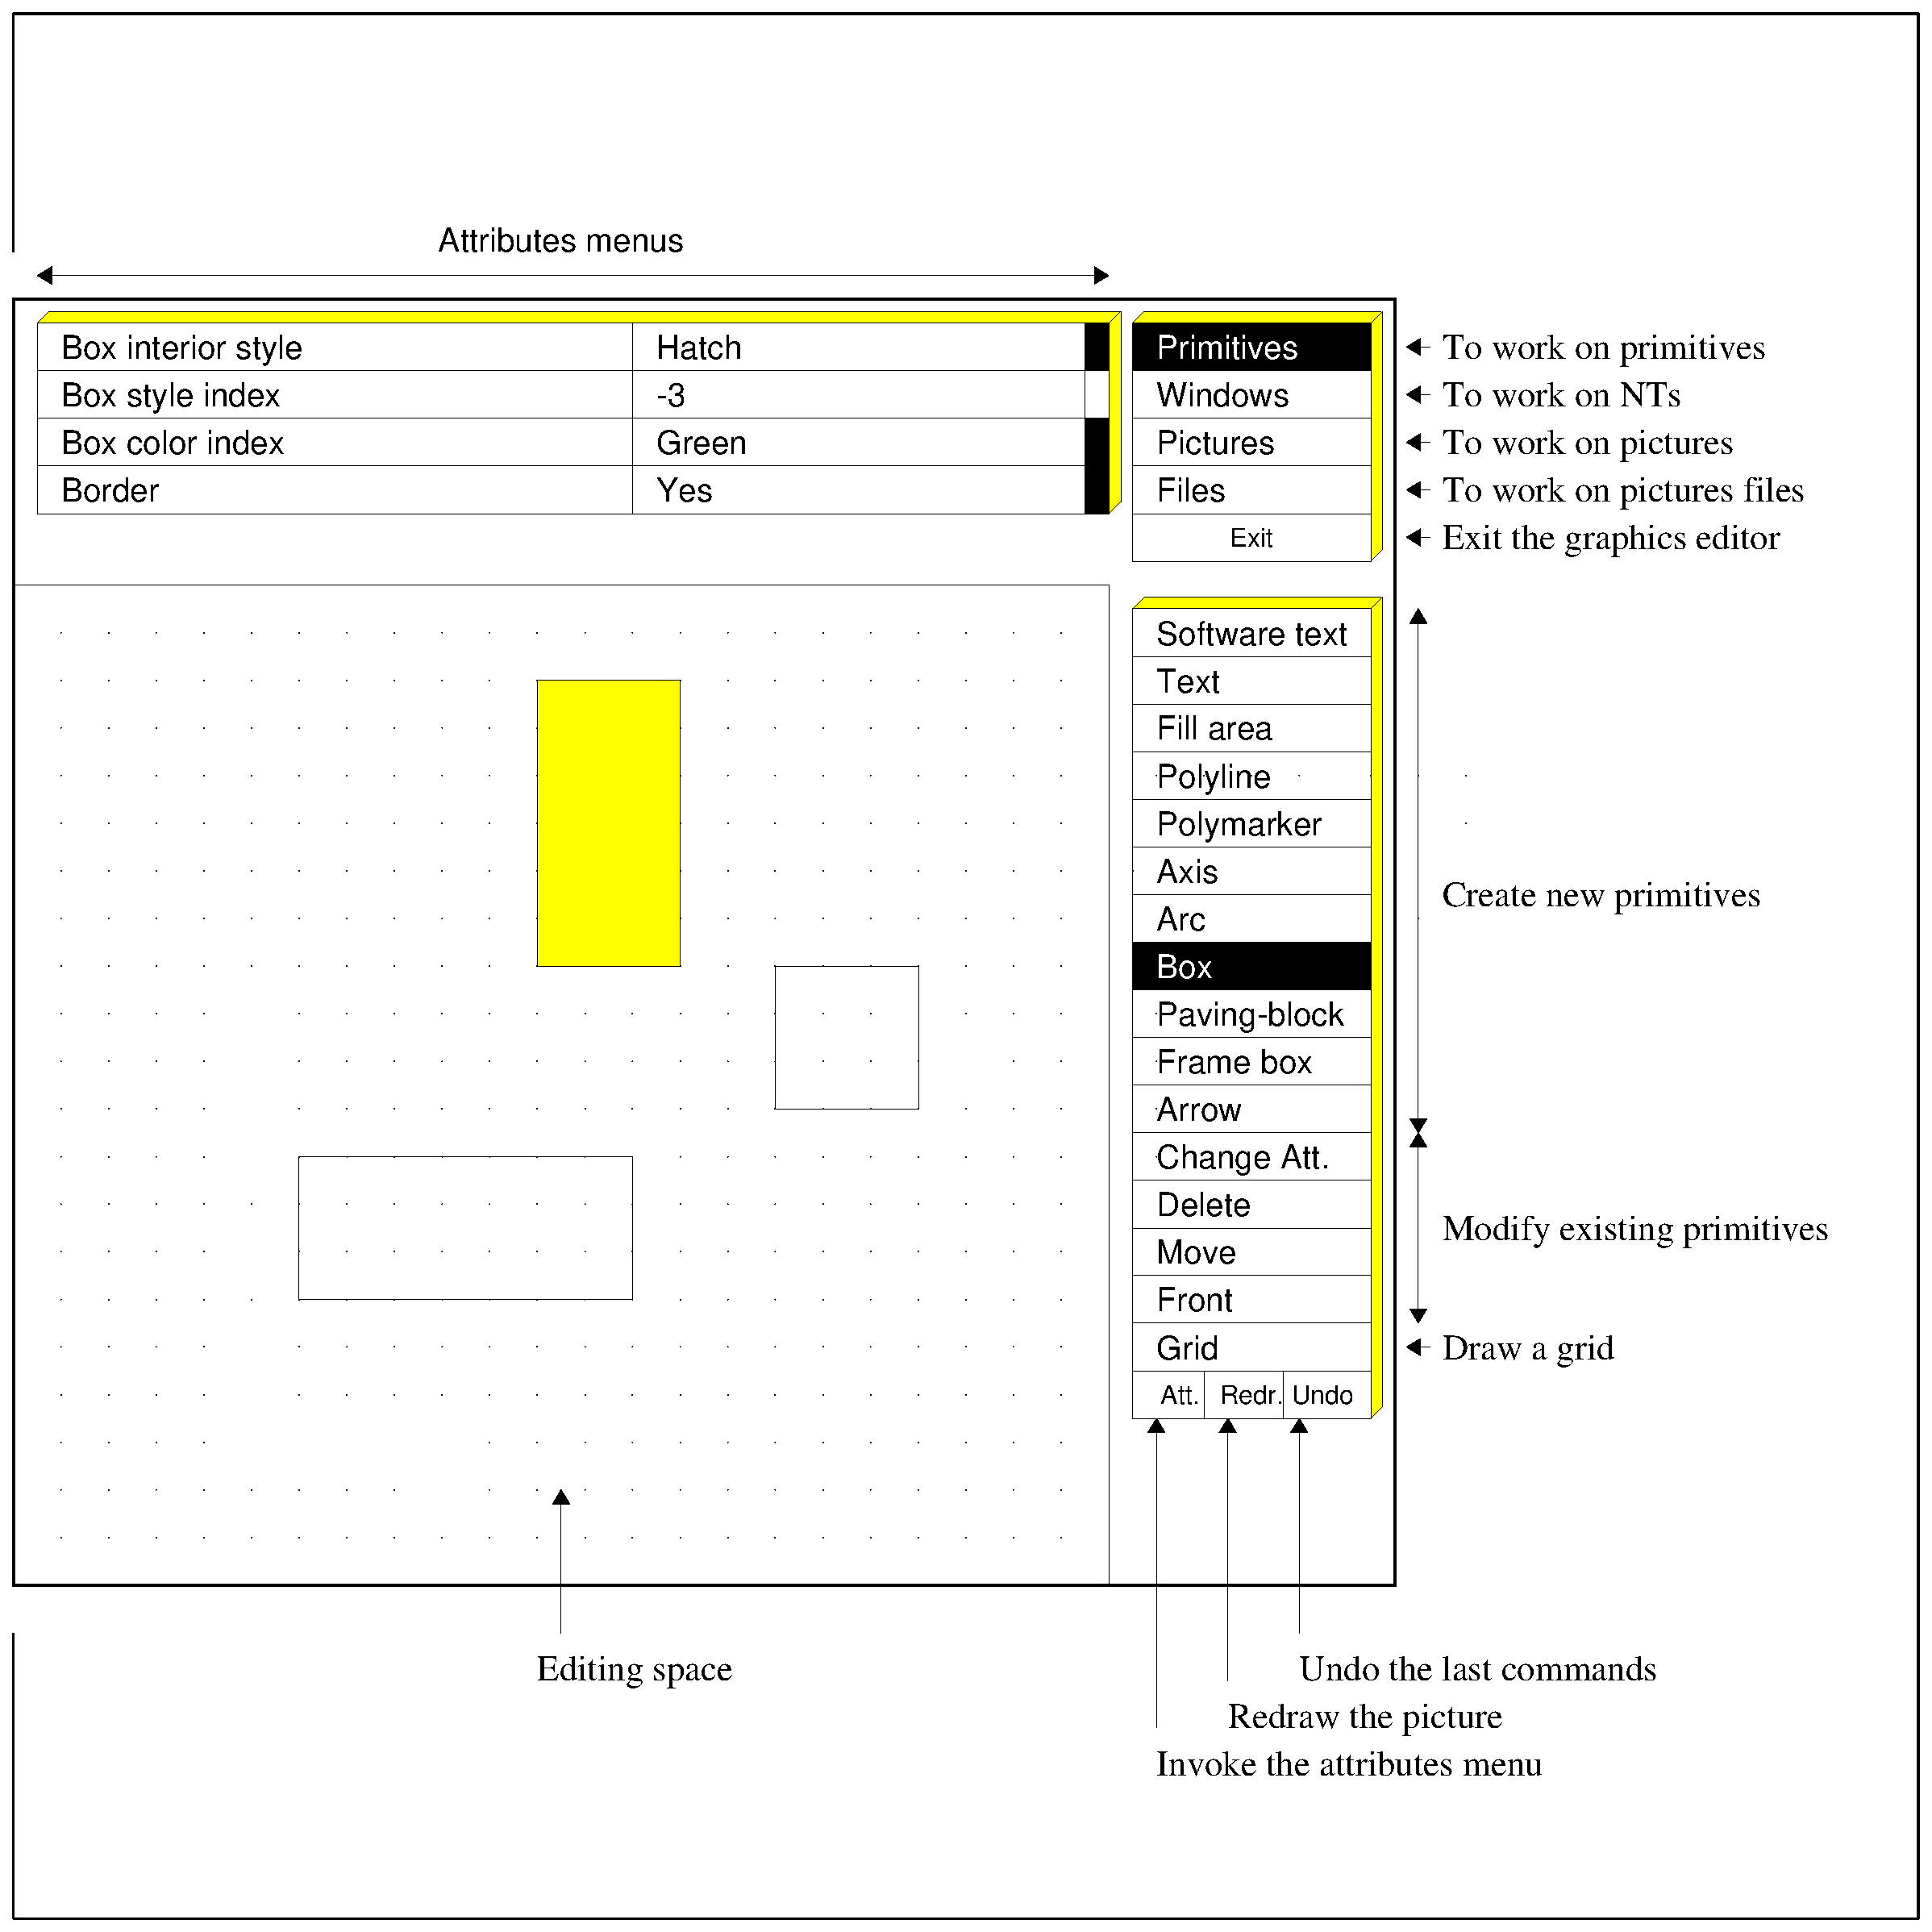
\epsfig{file=ged.eps,width=.9\textwidth}}
\end{center}
\caption{The graphics editor}
\label{fig-GED}
\end{Fighere}       
\end{minipage}
